\documentclass{article}
\usepackage[paperwidth=210mm,paperheight=297mm,top=20mm,bottom=20mm,left=20mm,right=20mm,headsep=0pt,headheight=0pt,footskip=0pt,marginparsep=0pt,marginparwidth=0pt,footnotesep=13.5pt plus 0.1pt minus 0.1pt]{geometry}
\usepackage[spanish,es-ucroman,es-noshorthands]{babel}
\usepackage[autostyle=true]{csquotes}
\tracinglostchars=2
\usepackage{fontspec}
\usepackage{microtype}
\newfontfeature{Microtypography}{protrusion=default;expansion=default}
\directlua{fonts.protrusions.setups.default.factor=.5}
\renewcommand{\normalsize}{\fontsize{10pt}{13.5pt}\selectfont}
\topskip=13.5pt
\setmainfont{Libertinus Serif}[Numbers={OldStyle,Proportional},Ligatures=TeX,Scale=1.2]
\setsansfont{IBMPlexSansCondensed}[Scale=MatchLowercase,Ligatures=TeX,Extension=.otf,UprightFont=*-Regular,ItalicFont=*-Italic,BoldFont=*-SemiBold,BoldItalicFont=*-SemiBoldItalic]
\setmonofont{IBMPlexMono.otf}[Scale=0.91,Extension=.otf,UprightFont=*-Regular,ItalicFont = IBMPlexMono-Italic.otf,BoldFont = IBMPlexMono-Bold.otf,BoldItalicFont = IBMPlexMono-BoldItalic.otf]
\usepackage{graphicx}
\usepackage{ragged2e}
\usepackage{xcolor}
\definecolor{color2}{RGB}{144,12,63}
\pagecolor{color2!1}
\usepackage[absolute]{textpos}
\newcommand\cabecera[1]{\sf\normalsize{#1}}
\newcommand\titulo[1]{\sf\LARGE{\textbf{#1}}}
\newcommand\subtitulo[1]{\sf\Large{#1}}
\newcommand\autoria[1]{\color{color2}\sf\Large{#1}}
\newcommand\legales[1]{\sf\normalsize{#1}}
\newcommand\texto[1]{\normalsize{#1}}
\newcommand\biografia[1]{\sf\small{#1}}
\usepackage{url}
\def\UrlFont{\tt\footnotesize}
\begin{document}
\thispagestyle{empty}
\begin{textblock*}{45mm}(15mm,20mm)
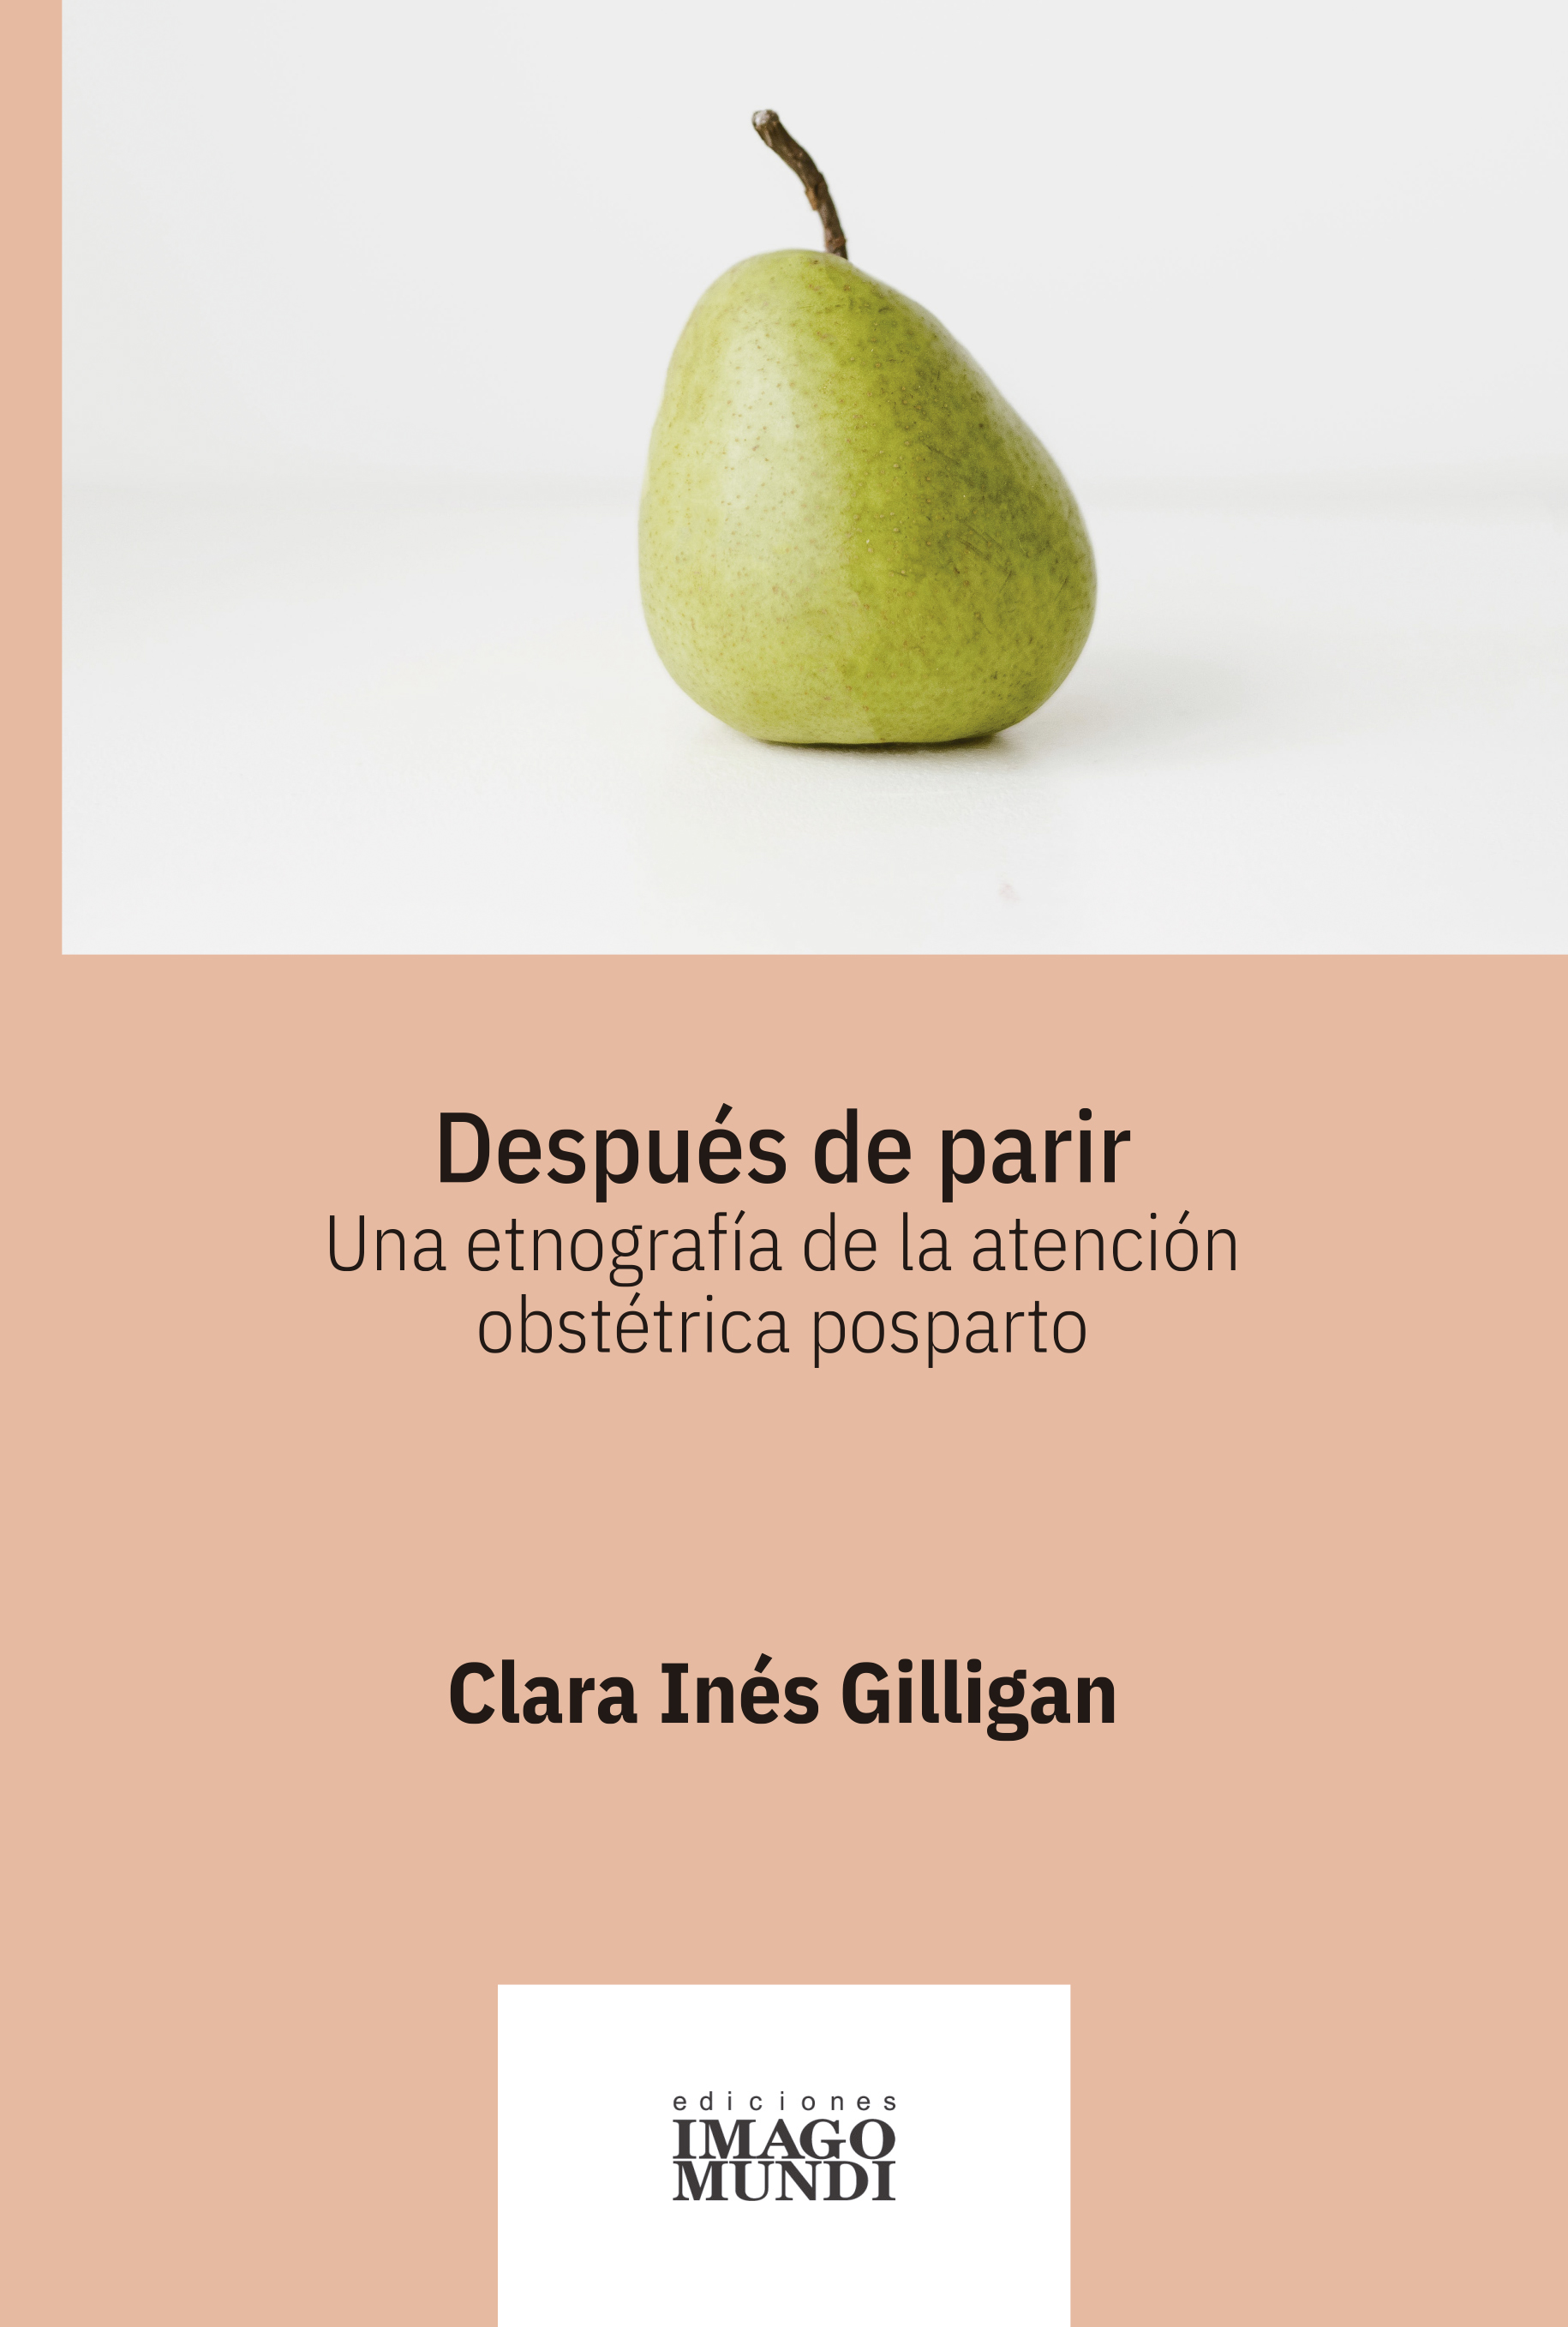
\includegraphics[width=45mm]{/home/alberto/Disco_Bodega/02_Produccion/00_Ejercicios/00-CharlaUBA/media/cover.png}
\end{textblock*}
\begin{textblock*}{45mm}(15mm,100mm)
\begin{minipage}{45mm}
\noindent\legales{ISBN: \textbf{0000}}\\
\noindent\legales{Formato: \textbf{15.5x23cm}}\\
\noindent\legales{Páginas: \textbf{999}}\\
\noindent\legales{Idioma: \textbf{es-ES}}\\
\noindent\legales{Fecha: \textbf{2024-01}}\\
\end{minipage}
\end{textblock*}
\begin{textblock*}{11cm}(75mm,20mm)
\begin{minipage}{11cm}
\noindent \cabecera{Colección {\color{color2}\textbf{Bitácora Argentina}}}\\
\noindent \cabecera{Dirigida por \textbf{Alejandro Daniel Falco}}\\
\end{minipage}
\end{textblock*}
\begin{textblock*}{11cm}(75mm,45mm)
\begin{minipage}{11cm}
\raggedright \titulo{III Jornada Latinoamericana de Estudios Editoriales}\\
\raggedright \subtitulo{Por la educación pública y el derecho a la enseñanza universitaria}
\end{minipage}
\end{textblock*}
\begin{textblock*}{11cm}(75mm,100mm)
\begin{minipage}{11cm}
\noindent \texto{Non eram nescius, Brute, cum, quae summis ingeniis exquisitaque doctrina philosophi Graeco sermone tractavissent, ea Latinis litteris mandaremus, fore ut hic noster labor in varias reprehensiones incurreret. nam quibusdam, et iis quidem non admodum indoctis, totum hoc displicet philosophari. quidam autem non tam id reprehendunt, si remissius agatur, sed tantum studium tamque multam operam ponendam in eo non arbitrantur. erunt etiam, et ii quidem eruditi Graecis litteris, contemnentes Latinas, qui se dicant in Graecis legendis operam malle consumere. postremo aliquos futuros suspicor, qui me ad alias litteras vocent, genus hoc scribendi, etsi sit elegans, personae tamen et dignitatis esse negent. Contra quos omnis dicendum breviter existimo. Quamquam philosophiae quidem vituperatoribus satis responsum est eo libro, quo a nobis philosophia defensa et collaudata est, cum esset accusata et vituperata ab Hortensio. qui liber cum et tibi probatus videretur et iis, quos ego posse iudicare arbitrarer, plura suscepi veritus ne movere hominum studia viderer, retinere non posse. Qui autem, si maxime hoc placeat, moderatius tamen id volunt fieri, difficilem quandam temperantiam postulant in eo, quod semel admissum coerceri reprimique non potest, ut propemodum iustioribus utamur illis, qui omnino avocent a philosophia, quam his, qui rebus infinitis modum constituant in reque eo meliore, quo maior sit, mediocritatem desiderent. Sive enim ad sapientiam perveniri potest, non paranda nobis solum ea, sed fruenda etiam [sapientia] est; sive hoc difficile est, tamen nec modus est ullus investigandi veri, nisi inveneris, et quaerendi defatigatio turpis est, cum id, quod quaeritur, sit pulcherrimum. etenim si delectamur, cum scribimus, quis est tam invidus, qui ab eo nos abducat? sin laboramus, quis est, qui alienae modum statuat industriae? nam ut Terentianus Chremes non inhumanus, qui novum vicinum non vult 'fodere aut arare aut aliquid ferre denique' -- non enim illum ab industria, sed ab inliberali labore deterret --, sic isti curiosi, quos offendit noster minime nobis iniucundus labor.}
\end{minipage}
\end{textblock*}
\begin{textblock*}{11cm}(75mm,77mm)
\begin{minipage}{11cm}
\noindent \autoria{Alberto Moyano}
\end{minipage}
\end{textblock*}
\begin{textblock*}{18cm}(15mm,277mm)
\begin{minipage}{18cm}
\centering
\url{https://gitlab.com/alberto.alejandro.moyano/CHARLAUBA}
\end{minipage}
\end{textblock*}
\end{document}

